\section{Introducción}
\subsection{Contexto}
	\begin{frame}{Actores}
		\begin{block}{Instituto de Salud}
			Realiza la solicitud de medicamentos mediante \textit{órdenes de reposición}.
		\end{block}
		\begin{block}{Sistema de Abastecimiento}
			Sistema web por el cual el Instituto de Salud realiza las órdenes de reposición.
		\end{block}
		\begin{block}{Farmacéutica}
			Quien provee medicamentos al Instituto de Salud.
		\end{block}
	\end{frame}

\subsubsection{Procesos}
	\begin{frame}{Envío de órdenes de reposición}
		\begin{figure}[H]
		\centering
		\includegraphics[width=\textwidth]{flow-proc-contestar} 
		\label{fig:flow-proc-contestar}
		\end{figure}
	\end{frame}

	\begin{frame}{Verificación de órdenes de reposición canceladas}
		\begin{figure}[H]
		\centering
		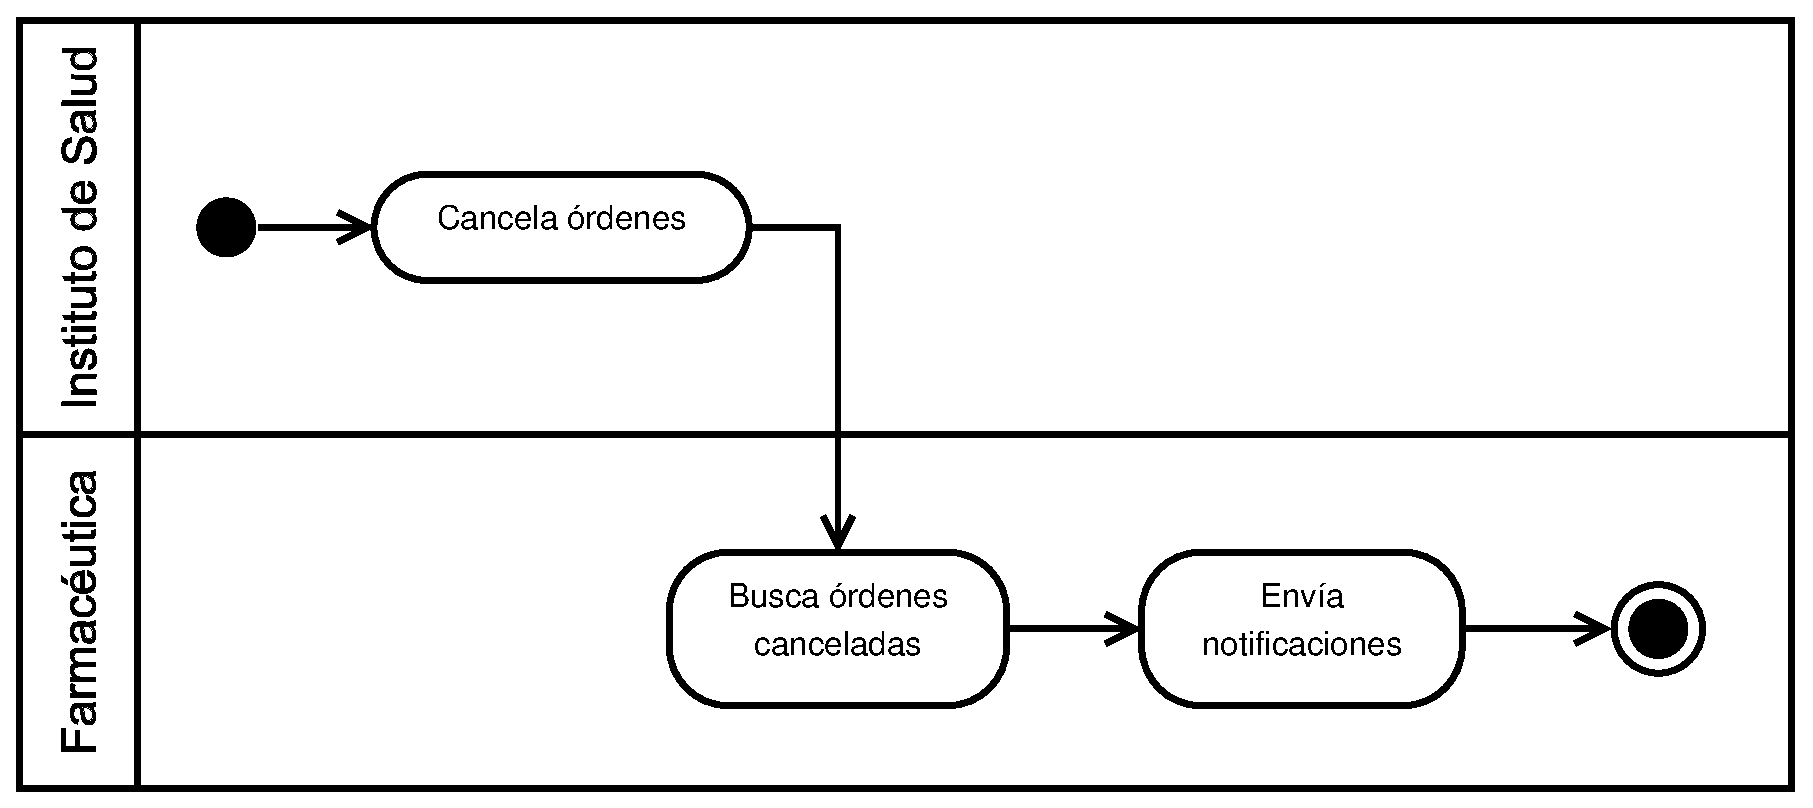
\includegraphics[width=\textwidth]{flow-proc-verificar} 
		\label{fig:flow-proc-verificar}
		\end{figure}
	\end{frame}

\subsection{Objetivos}
	\begin{frame}{Objetivo principal}
		Describir un sistema de cómputo que reduzca el tiempo de interacción entre los operadores de la farmacéutica y el \textit{Sistema de Abastecimiento}.
	\end{frame}

	\begin{frame}{Metas del objetivo principal}
		\begin{enumerate}
			\item Reducir el tiempo para contestar las órdenes de reposición.
			\item Evitar el envío de medicamentos no solicitados.
			\item Agilizar la generación de reportes.
		\end{enumerate}
	\end{frame}

	\begin{frame}{Objetivos secundarios}
		\begin{enumerate}
		\item Reducir el error humano en la manipulación de la información.
		\item Ahorrar recursos en la entrega de medicamentos no solicitados.
		\item Reducir el tiempo de respuesta a las órdenes de reposición.
		\item Dar consistencia en los datos de operación.
		\end{enumerate}
	\end{frame}

\subsection{Metodología de trabajo}
	\begin{frame}{Equipo de trabajo}
		\begin{block}{Metodología}
			Marco de trabajo \textit{Scrum}.
		\end{block}
		\begin{block}{Roles en el equipo de trabajo}
			\begin{enumerate}
				\item Arquitecto.
				\item Desarrollador.
			\end{enumerate}
		\end{block}
	\end{frame}

	\begin{frame}{Arquitecto}
		\begin{enumerate}
			\item Supervisar el diseño e implementación.
			\item Realizar investigación sobre herramientas.
			\item Cumplir con el rol de \textit{Scrum Master}.
			\item Formar parte del \textit{Scrum Team}.
		\end{enumerate}
	\end{frame}

	\begin{frame}{Desarrollador}
		\begin{enumerate}
			\item Levantar requerimientos.
			\item Realizar investigación sobre herramientas.
			\item Realizar diseño e implementación.
			\item Cumplir con el rol de \textit{Product Owner}.
			\item Formar parte del \textit{Scrum Team}.
		\end{enumerate}
	\end{frame}
